\textcolor{black}{\section{Anexo}}
% EJEMPLOS:
\begin{lstlisting}


\end{lstlisting}

\begin{figure}[H]
    \centering
    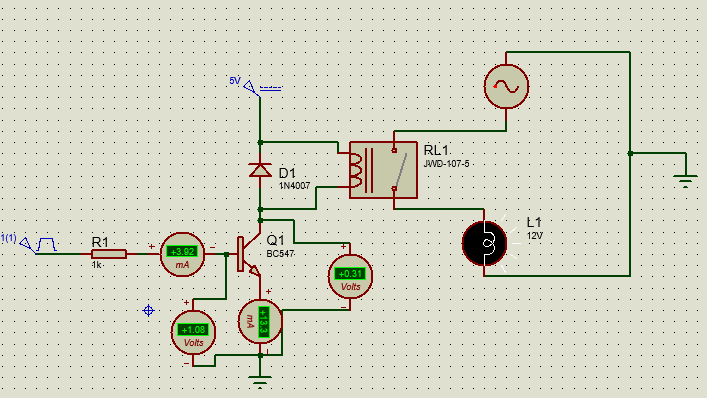
\includegraphics[scale=0.35]{figs/Circuito_1_simulado.png}
    \caption{Circuito eléctrico que controla el encendido y apagado de una lampara de corriente
alterna.}
    \label{Circuito1}
\end{figure}

\begin{figure}[H]
    \centering
    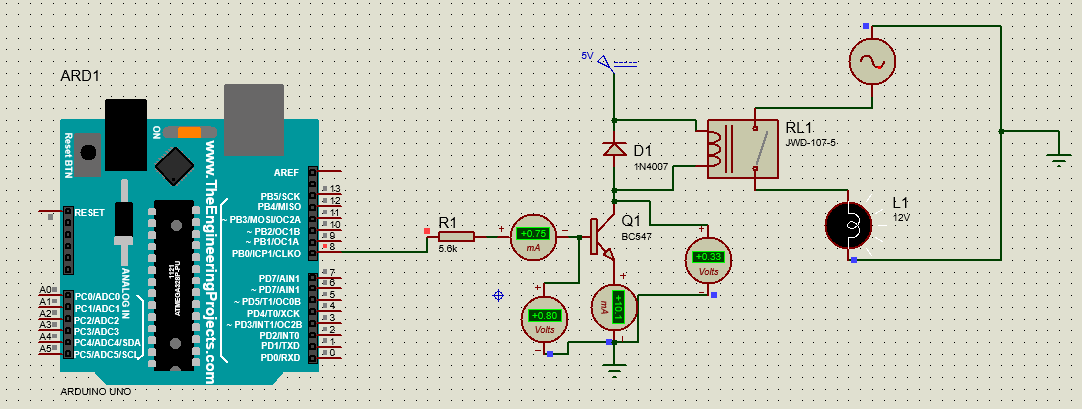
\includegraphics[scale=0.3]{figs/Circuito_2_simulacion.png}
    \caption{Circuito eléctrico que controla el encendido y apagado de una lampara de
corriente alterna utilizando Arduino.}
    \label{Circuito2}
\end{figure}

\begin{figure}[H]
    \centering
    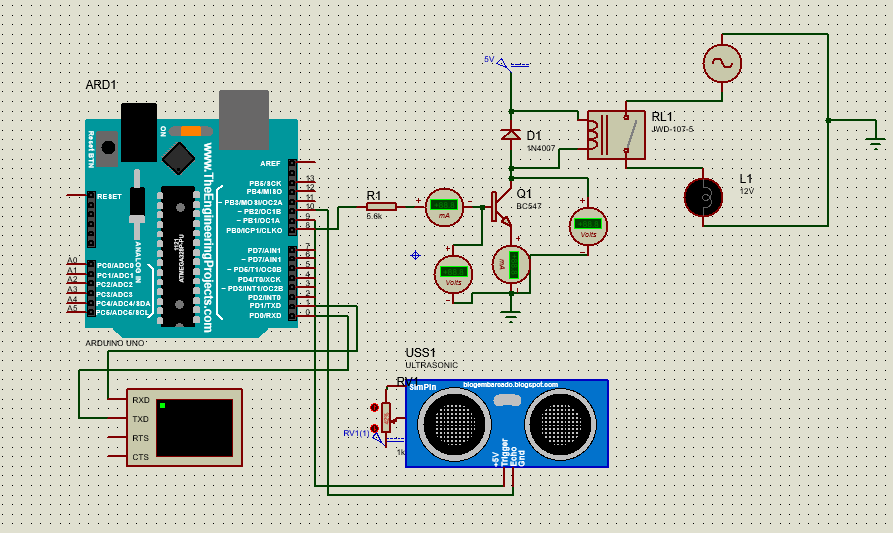
\includegraphics[scale=0.3]{figs/Circuito_3_simulado.png}
    \caption{Circuito eléctrico que controla el encendido y apagado de una lampara de
corriente alterna utilizando Arduino y un sensor de ultrasonido.}
    \label{Circuito3}
\end{figure}
% -----------------------------------------------

